\chapter{Automated modeling workflow in
Pirana}

\section{Background}\label{background}

An automated workflow alleviates the burden on modeling scientist by
removing the repetitive task of running and evaluating many candidate
models, standardizes the model development between modelers, and
standardize the results reported from such an analysis ultimately
leading to higher quality of PopPK analyses (\emph{Schmidt et al. JPKPD
2014 Aug}). In Pirana (version \textgreater{}= 2.10), such a workflow is
made available, and in this chapter we will walk through an example of
an automated population PK analysis.

\section{Tutorial}

For this chapter, we will use the template model library that is
provided with Pirana, and a (simulated) dataset of an iv-administered
drug also provided with Pirana (\texttt{demo.csv}).

\subsubsection*{Start}

Start Pirana Create a new project folder somewhere on your hard-drive
(or cluster). Browse into this folder (with Pirana). In this folder,
copy the file \texttt{demo.csv} that is included in the Pirana
installation folder (\texttt{Pirana/automod\_library/demo/demo.csv}). In
Pirana, go to \textbf{Tools} --\textgreater{} \textbf{Automated modeling
workflow}.


\subsubsection*{Screen 1: Models and
dataset}

\begin{figure}[htbp]
\centering
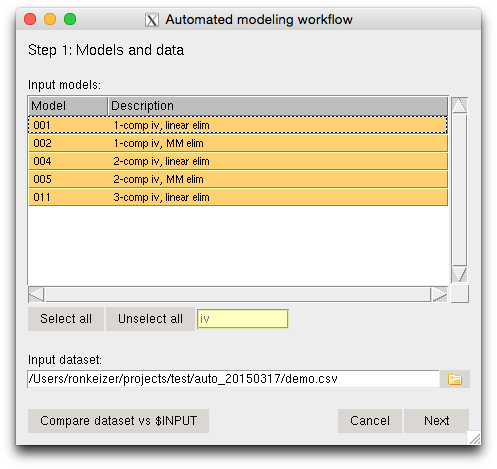
\includegraphics[scale=0.5]{images/screen1.png}
\caption{Screen 1: Models and dataset}
\end{figure}

This screen shows all models available in the library and which can be
selected to be included in the analysis. Use the filter for conveniently
selecting e.g.~only \emph{iv} or only \emph{oral} models. The dataset
should of course be specified as well before you can advance to the next
step. By default, it will use the first \texttt{.csv} file in this
folder (in alphabetic order).

When models and dataset have been selected, you should check whether the
\texttt{\$INPUT} record in the models matches with the headers in the
dataset. For this, click the button \texttt{Compare dataset vs}\$INPUT`.
This will bring up screen shown in figure 2:

\begin{figure}[htbp]
\centering
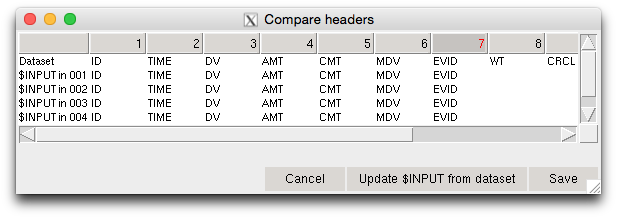
\includegraphics[scale=0.5]{images/compare.png}
\caption{Compare/set input headers}
\end{figure}

If the \texttt{\$INPUT} in the models (shown in rows 2-\ldots{}) does
not match up with the dataset (shown in row 1), you can click the button
\texttt{Update \$INPUT from dataset}. This will create a new \$INPUT
record for all models. After clicking \textbf{Save}, when the models
will be written (in step 3 of the automated analysis), the \$INPUT
records in all models will be changed to the new one. It is left to the
user to make sure that the variables used in the model are still
included in \$INPUT, as there is no extra check in place for that.

For our current analysis, we will select all \emph{iv} models, so filter
on \emph{iv}, and select the remaining models. Update the
\texttt{\$INPUT} records, click \emph{Save} and then \emph{Next} to
advance to the next step.


\subsubsection*{Screen 2: Setting initial parameter
estimates}\label{screen-2-setting-initial-parameter-estimates}

In the second screen, we can set initial parameter estimates, as well as
lower and upper bounds. All parameters are read from the models that
were selected in step 1. The parameter descriptions are defined in the
models as comments to \texttt{\$THETA}, \texttt{\$OMEGA}, and
\texttt{\$SIGMA} blocks, like e.g.

\begin{figure}[htbp]
\centering
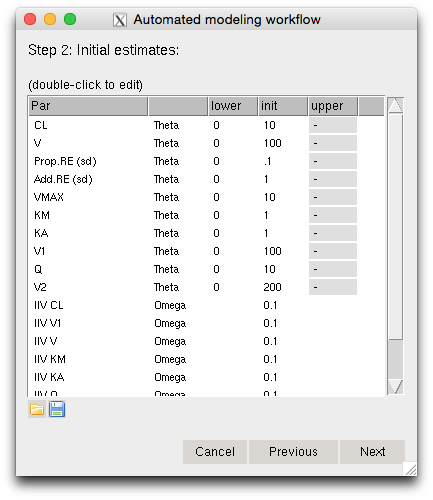
\includegraphics[scale=0.5]{images/screen2.png}
\caption{Screen 2: Initial parameter estimates}
\end{figure}

\begin{verbatim}
$THETA
(0, 5, 100); CL
(0, 5, 100); V

$OMEGA
(0.1); CL
(0.1); V

$SIGMA
0.05 ; proportional error
\end{verbatim}

\emph{Note:} At current, correlations in \$OMEGA and \$SIGMA cannot be
specified for an automated analysis. I.e. only the diagonal elements of
\$OMEGA and \$SIGMA can be specified in the template models if you want
to update them in this step. You can still include models that have full
\$OMEGA or \$SIGMA blocks as template model, however you cannot provide
descriptions (as comments) to the parameters in the block, and you
cannot update them in this step of the analysis.

The two buttons below the parameter grid can be used to save and
(re-)load parameter definitions to file.

For our analysis, let's leave the parameters as they are. Click
\textbf{Next} to advance to the next step.


\subsubsection*{Screen 3: Folders}\label{screen-3-folders}

\begin{figure}[htbp]
\centering
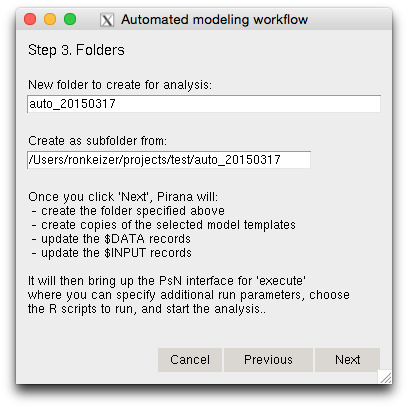
\includegraphics[scale=0.5]{images/screen3.png}
\caption{Screen 3: Folders}
\end{figure}

In this screen we can specify where to create the new models and run the
analysis. By default it will generate a new folder name based on the
current date, and as a subfolder from the current folder in Pirana. This
screen also lists the actions that Pirana will perform once you click
\emph{Next}.

Let's use the defaults and click \emph{Next}.


\subsubsection*{Screen 4: PsN dialog}\label{screen-4-psn-dialog}

\begin{figure}[htbp]
\centering
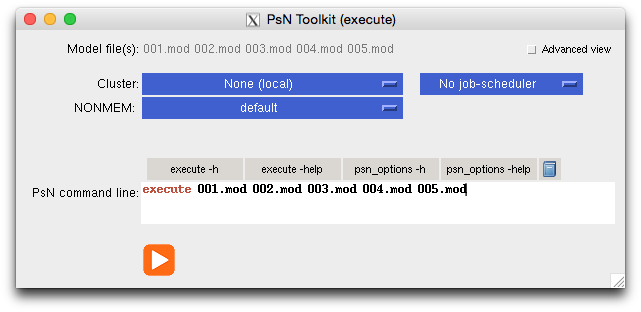
\includegraphics[scale=0.5]{images/psn_simple.png}
\caption{Screen 4: PsN}
\end{figure}

Pirana should now have switched automatically to the new folder where
you will see the newly generated models. Pirana will also automatically
bring up the PsN \texttt{execute} dialog. In this dialog, if you switch
to \textbf{Advanced view}, you can select which R script(s) to run after
all runs have been completed to generate goodness-of-fit plots. Click
the \emph{folder} icons next to the R scripts textboxes to select R
scripts (or batch files) to run after (or before) the analysis (figure
6).

\begin{figure}[htbp]
\centering
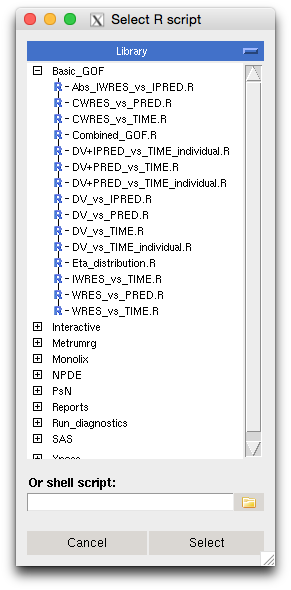
\includegraphics[scale=0.5]{images/run_r.png}
\caption{Select R script}
\end{figure}

For our analysis, we will select the \textbf{Basic GOF plots as single
doc} from the \texttt{Reports} folder to create GOF plots for all
models. The graphical report will automatically be opened, but is also
available from the \emph{Reports} tab on the right.

If you have not selected R scripts to be executed automatically after
the analysis has completed, you can still create them afterwards by
selecting the runs and running any R script from the \textbf{R} tab on
the right side of the Pirana window.

Besides the graphical report, Pirana can generate a \emph{numeric}
report for the analysis, including e.g.~OFVs, basic run information and
parameter estimates. This document is not generated automatically but
has to be requested manually after the analysis is complete: Make sure
Pirana is still in the folder where the analysis was run, and then go to
\textbf{Tools} --\textgreater{} \textbf{Automated modeling workflow}
--\textgreater{} \textbf{Report}. On the first page you will see an
overview of all models included in the analysis and their respective
OFV, AIC and BIC (figure 7). The subsequent pages includes information
on each individual run in the analysis.

\begin{figure}[htbp]
\centering
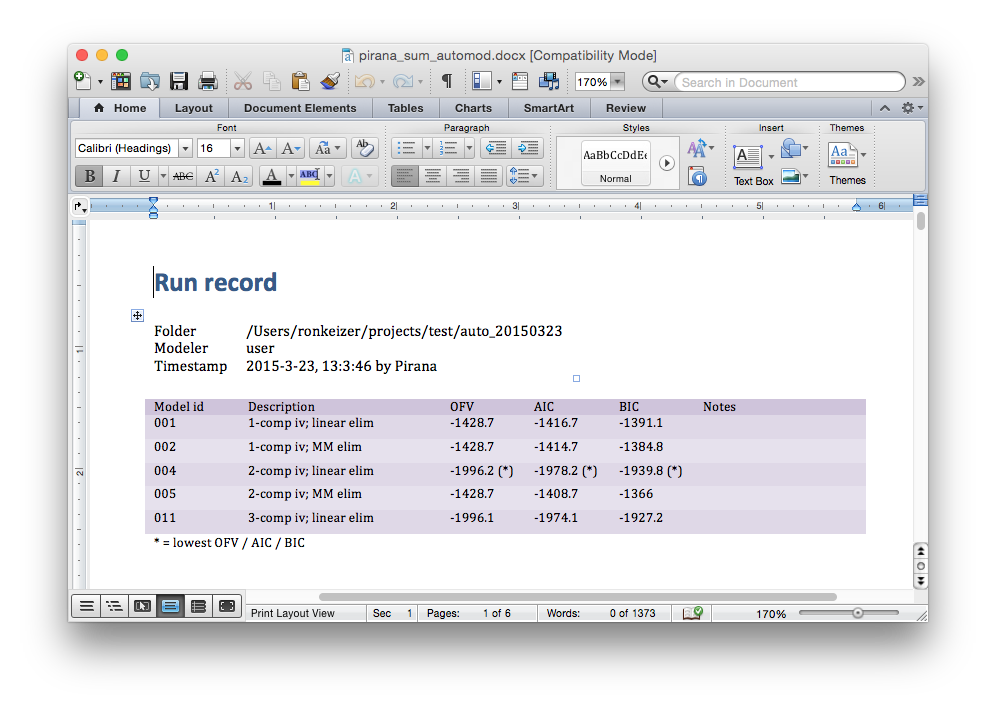
\includegraphics[scale=0.5]{images/report.png}
\caption{Report in Word}
\end{figure}
